\section{Implementazione}
\begin{frame}{Implementazione}
    Per implementare un servizio onion è necessario utilizzare un \textbf{Proxy Onion} per inoltrare le richieste dalla rete Tor al server web. Il proxy gestisce la generazione delle chiavi, dell'indirizzo e la definizione e connessione con gli \textbf{introduction points}, oltre alla generazione del descriptor e la sua pubblicazione nei Directory Servers. \\
    In particolare la nostra implementazione \textbf{Onion V3} (dato che Onion V2 è stato deprecato) userà un server \textbf{Linux} su AWS per ospitare il Proxy Onion e un \textbf{server nginx}.
\end{frame}

\begin{frame}
    Nel sistema è necessario installare il web server NGINX e dopo una serie di configurazioni dei repository possiamo installare il Proxy Tor. Nel file di configurazione \hyperref[torConfig]{torrc} è possibile indicare la directory in cui salvare le chiavi e il tipo di connessione con il web server. \\
    In questa implementazione ho usato un tool (\href{https://github.com/cathugger/mkp224o/}{mkp224o}) per generare la coppia chiave privata e pubblica che risulti in un indirizzo onion personalizzato.
\end{frame}

\begin{frame}
    \centering
    \href{http://tesilm3jb64lw3upj4uu5fsxi2nrtbhbhkbu2dsbn46qka7j4kf7peqd.onion}{http://tesilm3jb64lw3upj4uu5fsxi2nrtbhbhk bu2dsbn46qka7j4kf7peqd.onion}
    \begin{figure}
        \centering
        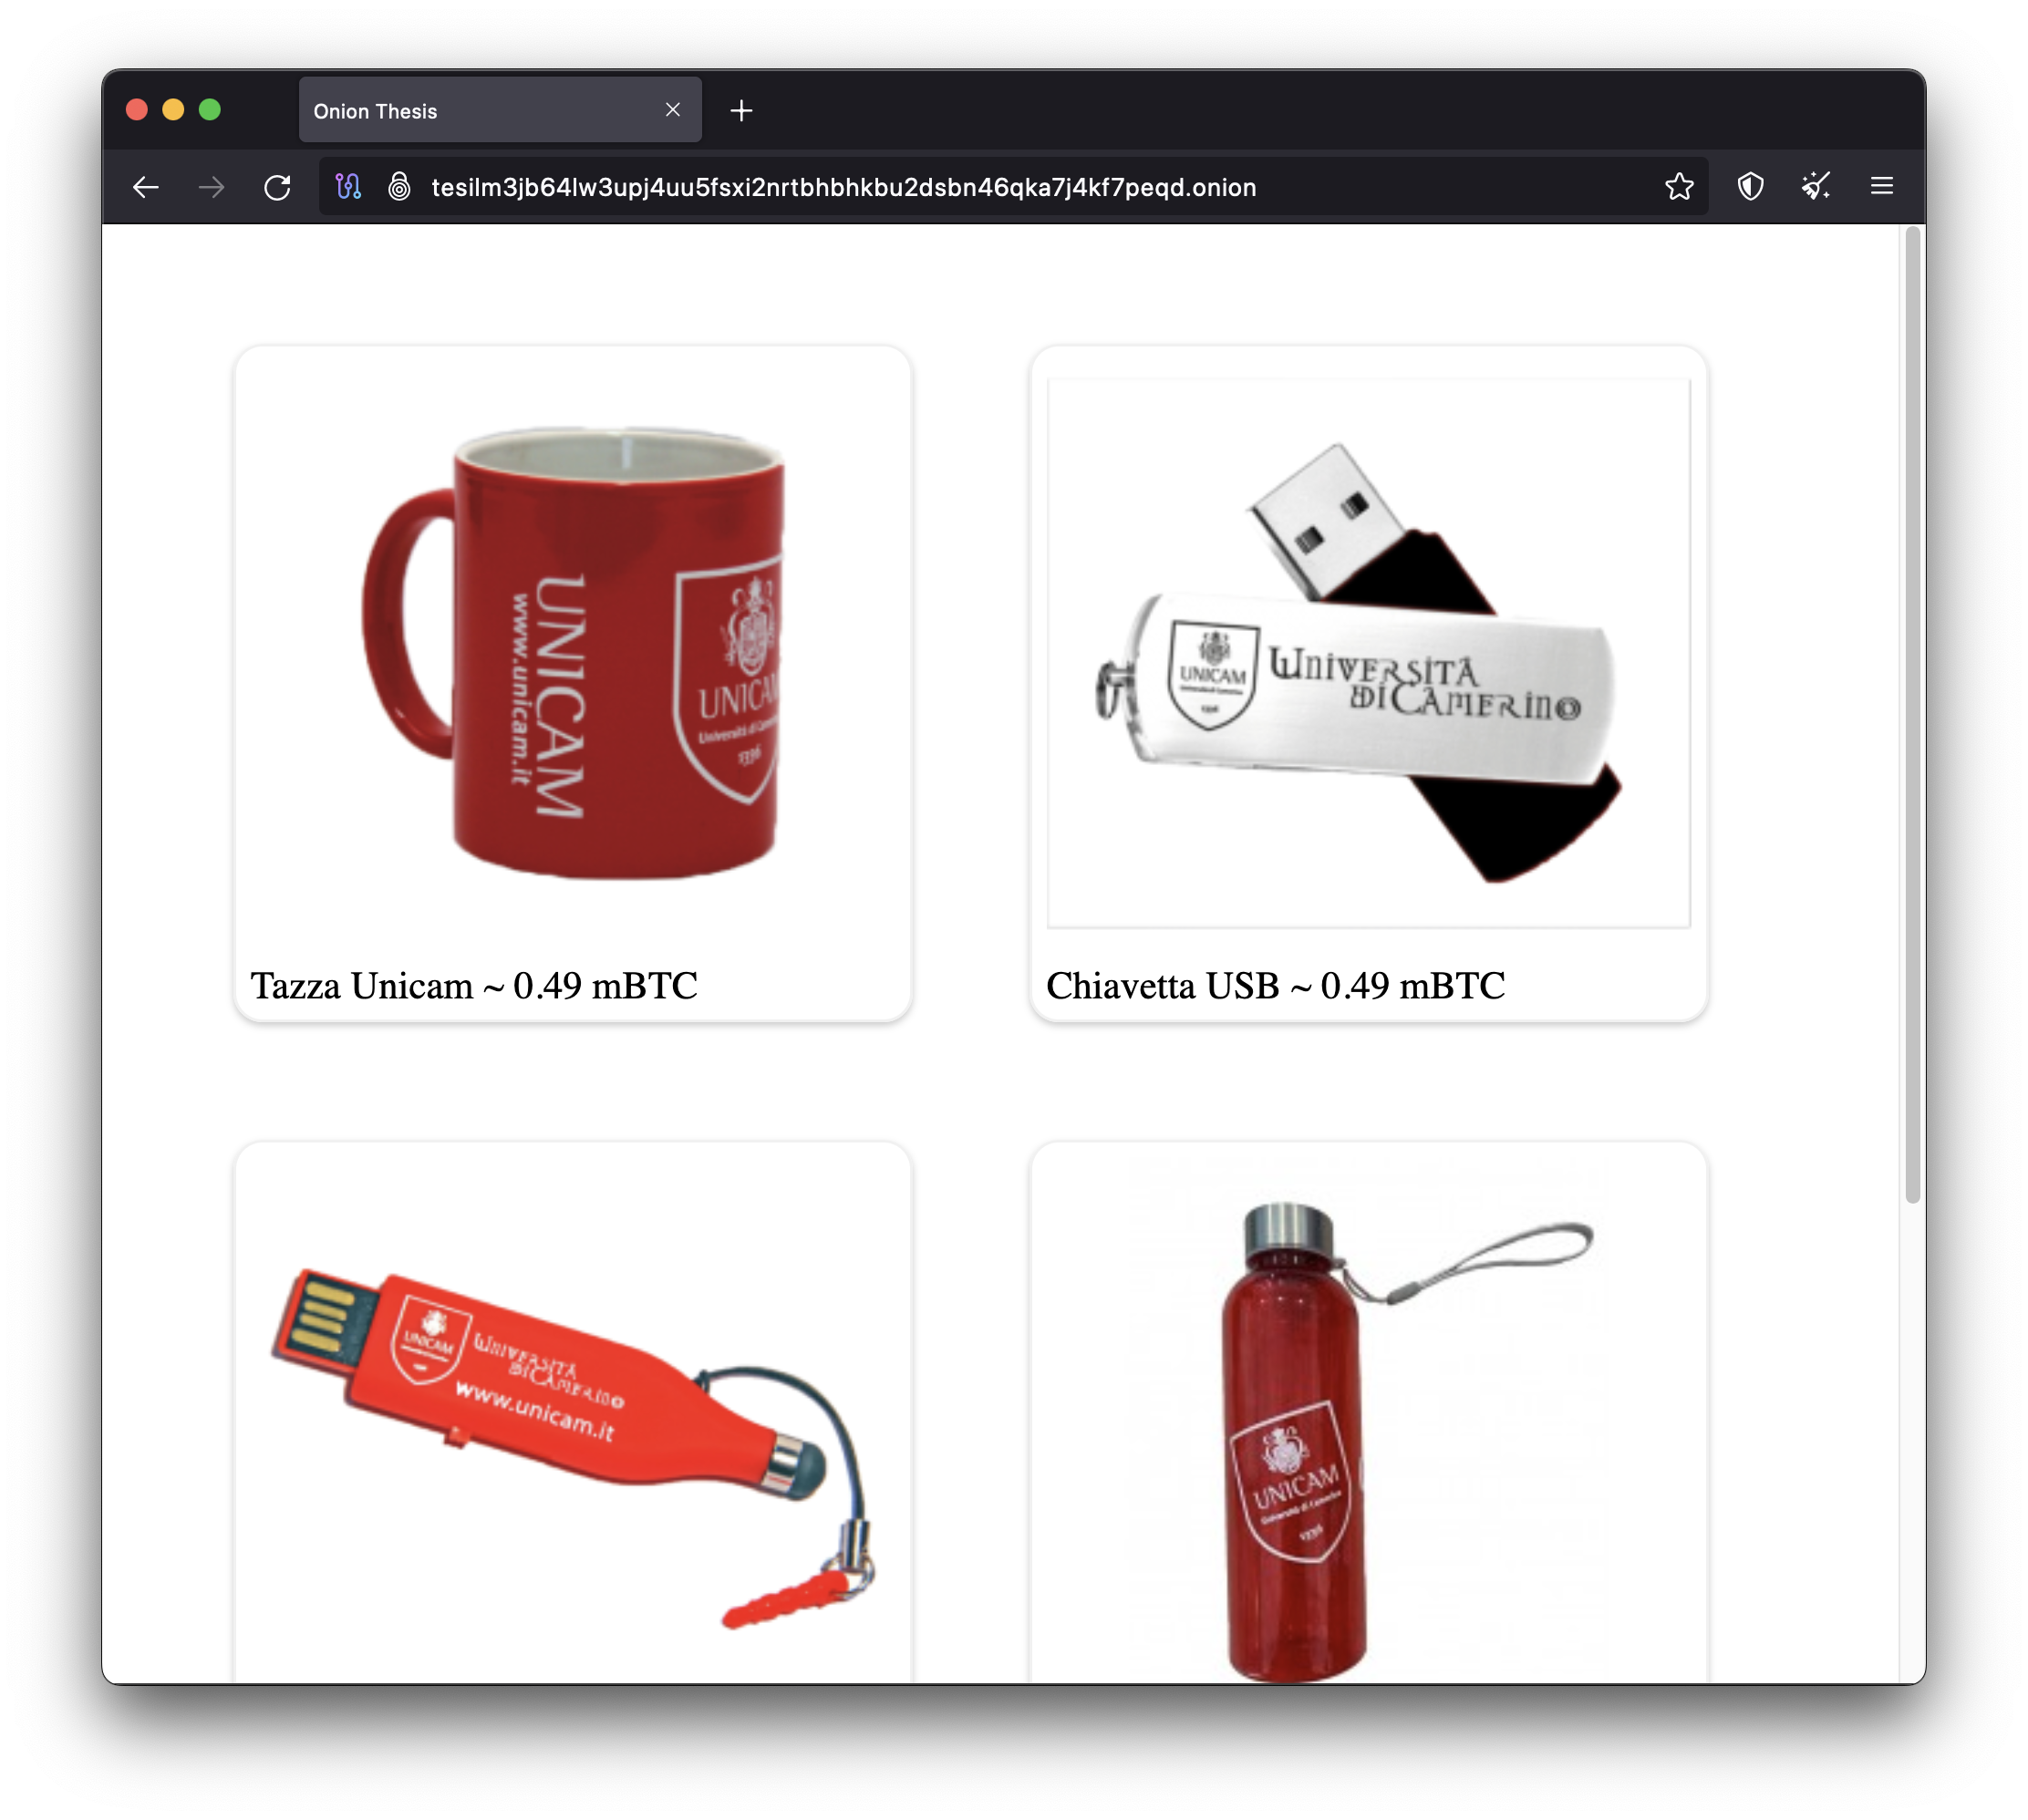
\includegraphics[width=0.8\textwidth]{OnionConnection.png}
    \end{figure}
\end{frame}

\subsection{Pubblicizzare il servizio}
\begin{frame}{Pubblicizzare il servizio}
    Nel lavoro di tesi abbiamo mostrato come pubblicizzare il servizio onion tramite un'\textbf{Header Tag}, è infatti possibile inserire un tag all'interno della pagina html che quando aperto con Tor consente di reindirizzare l'utente al relativo sito onion.
    \href{http://tesilm3jb64lw3upj4uu5fsxi2nrtbhbhkbu2dsbn46qka7j4kf7peqd.onion}{\lstinline{<meta http-equiv="onion-location" content="http://tesilm3jb64lw3upj4uu5fsxi2nrtbhbhkbu2dsbn46qka7j4 kf7peqd.onion" />}}
    % The space is important to make the line break correctly
\end{frame}

\begin{frame}
    \begin{figure}
        \centering
        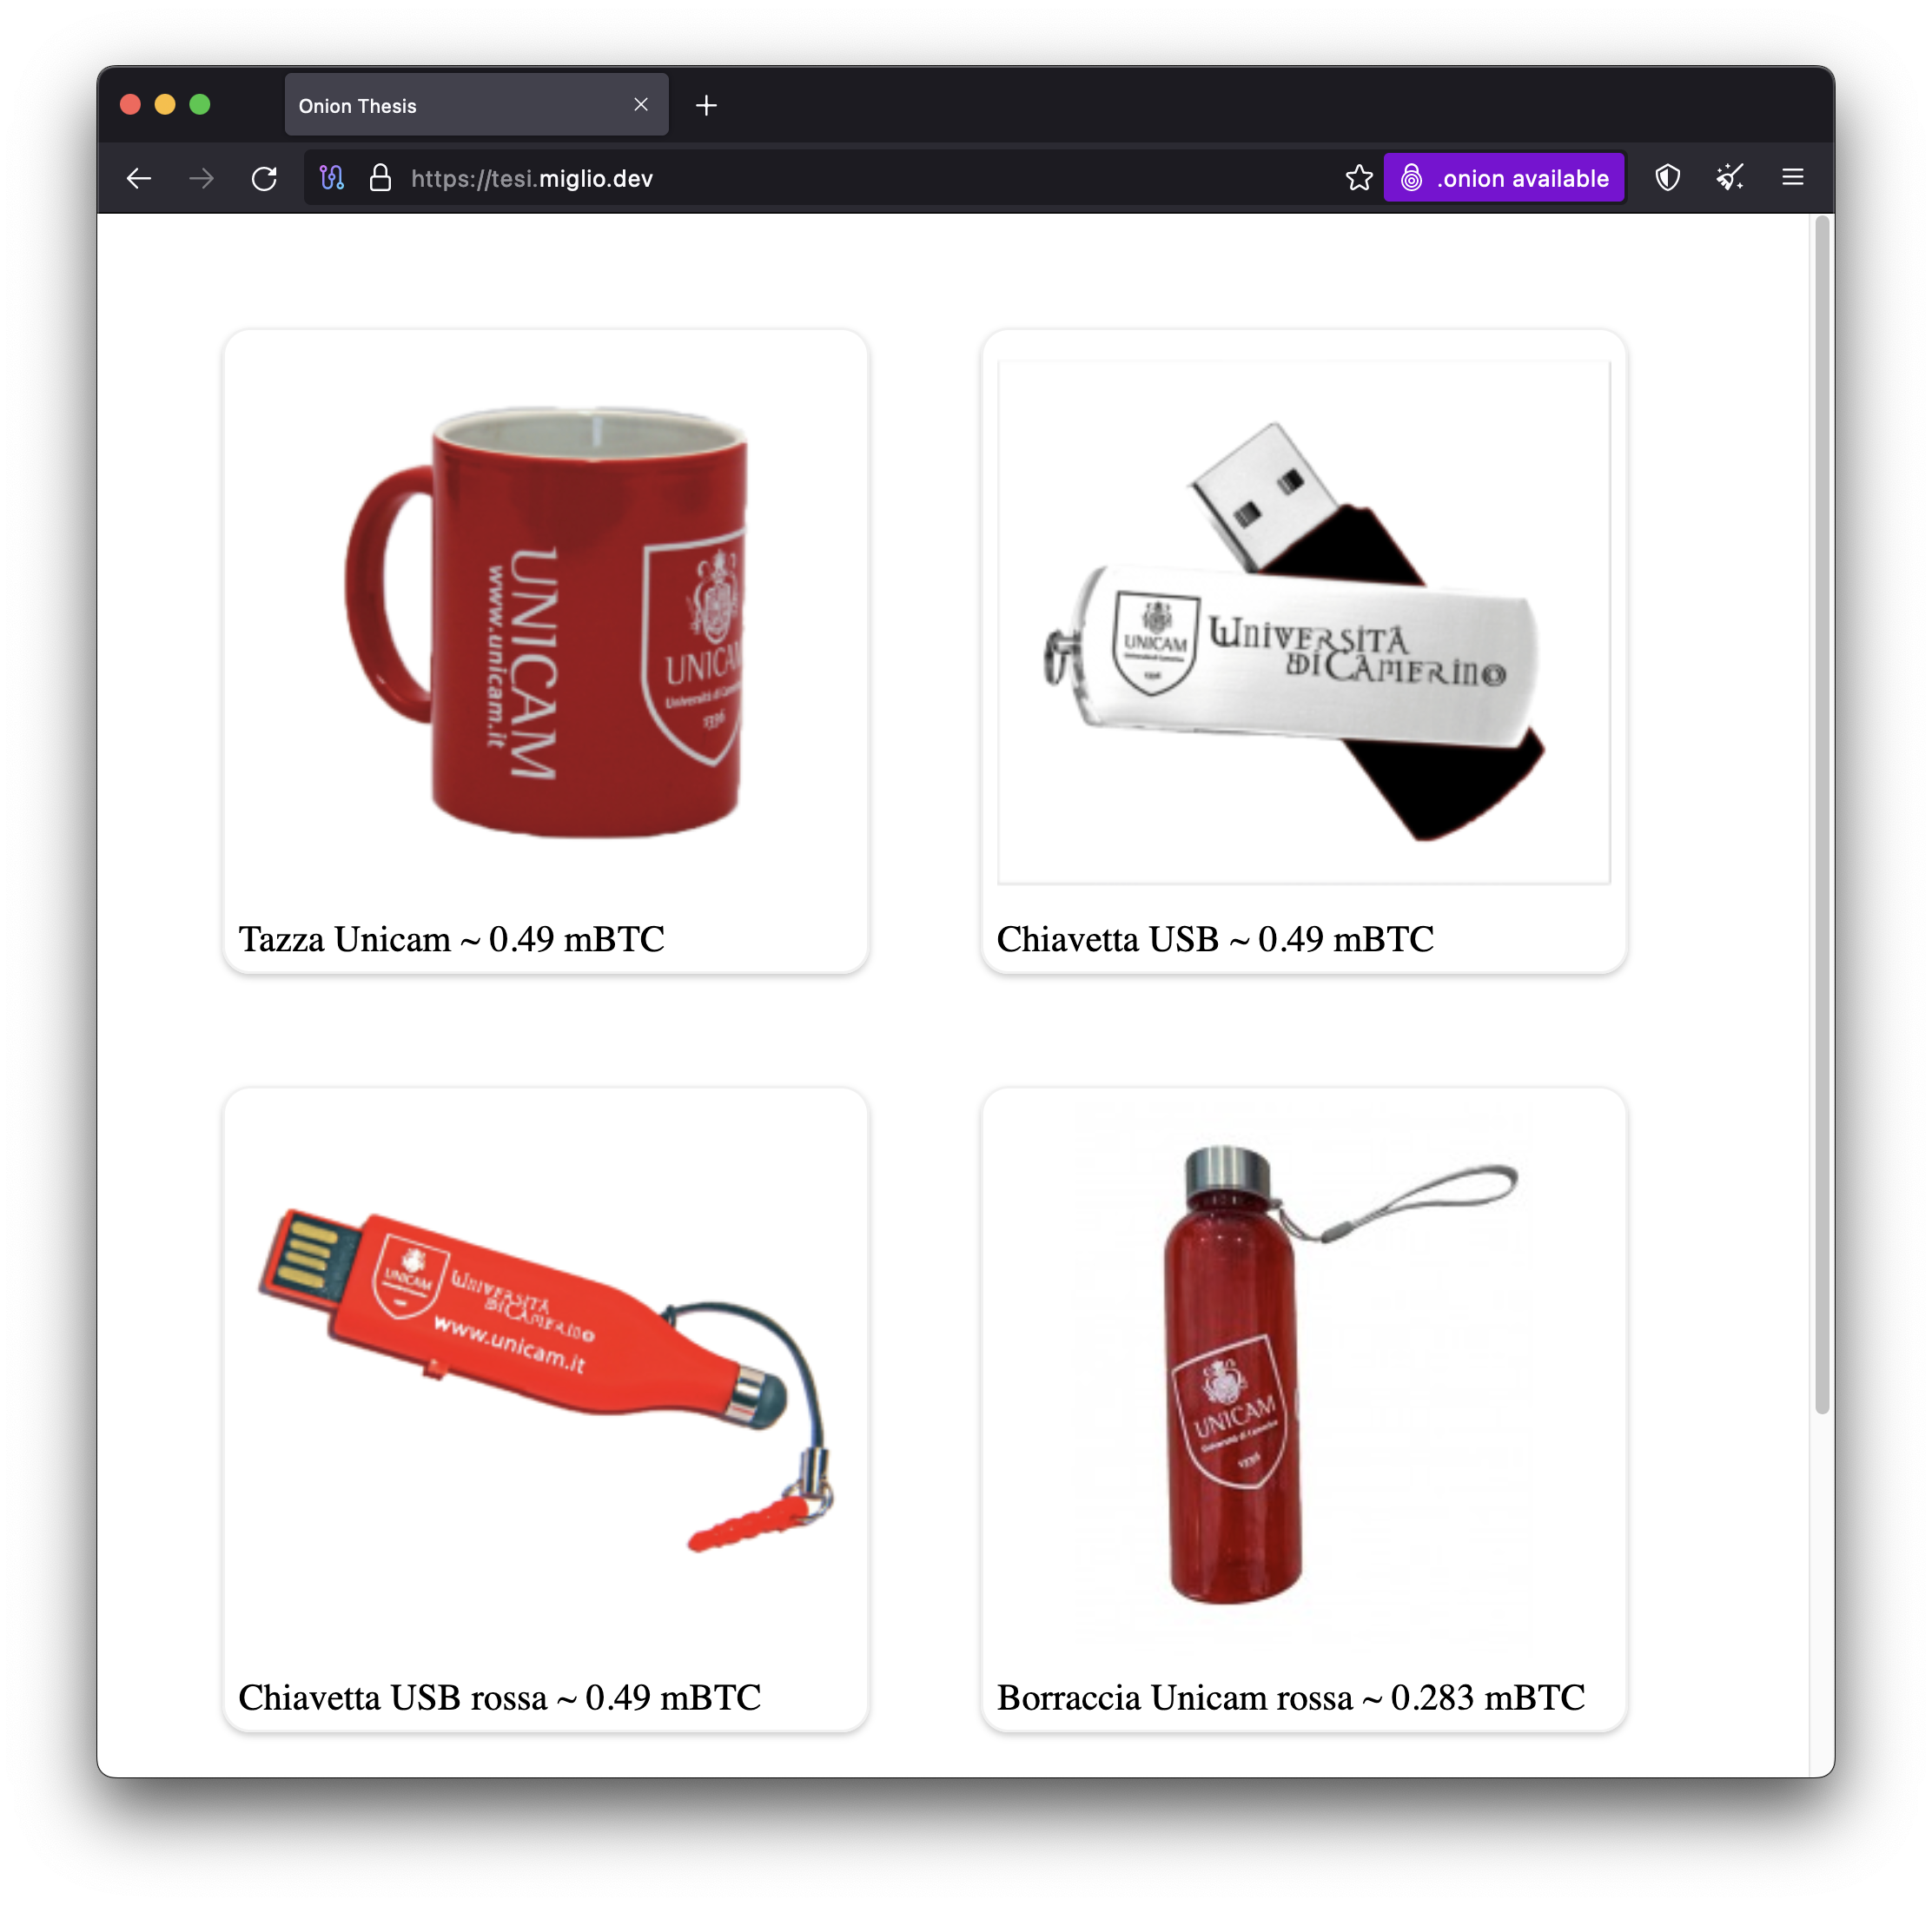
\includegraphics[width=0.8\textwidth]{ClearWebPage}
    \end{figure}
\end{frame}

